\documentclass[11pt]{scrreprt}
\usepackage[utf8]{inputenc}
\usepackage{graphicx}
\usepackage{longtable}
\usepackage{multicol}
\usepackage{booktabs} % http://ctan.org/pkg/booktabs
\usepackage[numbib]{tocbibind} % http://www.ctan.org/pkg/tocbibind

\newcommand{\tabitem}{~~\llap{\textbullet}~~}
\newcommand*{\SignAndDate}[1]{%
    \par\noindent\makebox[2.5in]{\hrulefill} \hfill\makebox[2.0in]{\hrulefill}%
    \par\noindent\makebox[2.5in][l]{#1}      \hfill\makebox[2.0in][l]{Date}%
}%

\title{\textbf{Clang AST Analysis and Repair}}
\subtitle{2014-2015 Computer Science Capstone Project}
\author{Nicholas Nelson\\
		Charles Santos}
\date{}
\begin{document}

\maketitle

\tableofcontents

\chapter{Project Introduction}

This project was requested by Garmin AT Inc., a subsidiary of Garmin Corporation, as part of their ongoing commitment to engineering education at Oregon State University and the continued growth of software engineering requirements within their internal software development teams.

Garmin AT focuses on avionics and navigational electronics for use within private and commercial aircraft.
This equipment contains embedded firmware and software written in C and requiring exacting standards and precision under Federal Aviation Administration (FAA) guidelines prior to use in production products.
Combining these FFA standards with Garmin AT's internal style and formatting guidelines has meant that evaluating and fixing compliance issues has been a time consuming process.

The purpose of this project was to use an internally developed code review tool as a baseline to develop a modular application that leverages the LLVM project's Clang AST interpreter libraries\footnote{http://clang.llvm.org/} and the Python regular expression libraries to process rulesets for each style and formatting requirement.

The project team consisted of Andrew Stucky, Embedded Software Engineer at Garmin AT, Nicholas Nelson and Charles Santos, both of whom are senior Computer Science students at Oregon State University.
As the project sponsor and mentor, Andrew provided the project requirements, initial codebase, and testing infrastructure.
Nick Santana, a member of Andrew's development team, provided support for the runtime codebase and assisted with the integration of changes to the infrastructure that runs the rulesets.

The entire project codebase was maintained on GitHub\footnote{https://github.com/}, and utilized the project management capabilities of that platform.
The project was designed in a modular fashion to allow individual formatting rules to be developed and tracked in separate branches.
Issues for each rule, submitted by Andrew, were used to document requirements, design decisions, team communications, and status updates.
Pull requests between development branches and the master branch were used to alert Andrew that a potential solution to a specific rule was ready for final testing and integration into the codebase that would be included in one of three major version releases that occurred during the project.

\chapter{Original Client Requirements Document}

\section{Introduction}
Garmin AT develops navigational components for a variety of aircraft. These components provide a high degree of situational awareness to pilots by integrating data from a variety of sources including GPS, weather, and traffic information from the Automatic Dependent Surveillance-Broadcast (ADS-B) data link network. Avionics displays similar to the products Garmin produces were crucial to the Capstone Program in Alaska which reduced accidents state wide by 40\% from 1999 to 2009 according to a report published by the Federal Aviation Administration.

Avionics software must meet Federal Aviation Administration (FAA) guidelines for safety and operations certification, specifically DO-178B/ED-12B (Software Considerations in Airborne Systems and Equipment Certification), prior to being allowed within any operational aircraft.

Garmin AT currently utilizes Python regular expression scripts for internally evaluating code quality and standards prior to submitting for FAA certification. We have been tasked with reimplementing and expanding functionality to take advantange of the Clang AST parser library. These changes will allow more complex rulesets that can flag potential syntax irregularities and automatically correct them if possible; or allowing for human review otherwise.

\section{Project Description}
Garmin’s avionics products are powered by embedded firmware and software written in C. There are serious safety considerations for any code embedded in avionics components; a bug at the wrong time could result in serious injury or death to the pilot and passengers of the craft relying on this software. Therefore embedded avionics software must follow precise quality control guidelines established by the FAA. Garmin also has internal style and formatting guidelines that they would like to enforce. Garmin has automated some quality control for these guidelines using regular expressions. However regular expressions are difficult to maintain and many of the rules are not easily implemented using regular expressions. Now Garmin is looking to implement these rules using python scripts and to create scripts for many of the rules that have not yet been implemented using regular expressions.

Our scripts will be examining abstract syntax trees to determine if the source code is compliant with FAA and Garmin guidelines. We will be using abstract syntax trees provided by Clang to examine C source code using python scripts. When a script finds a violation of the guidelines it will either make the necessary change or alert the user to the problem.

The client has provided us with the list of rules/issues that need to be implemented in python in rule specific scripts. There may be a number of issues that are more appropriate as regular expressions and that will have to be determined as we progress and consult with the client. Some of these python scripts may group together multiple issues that are related. Users will specify C source/header files that need to be checked, our main script will use Clang to parse the abstract syntax trees from these files. The main script will then call scripts for each of the rule specific scripts which will examine the ASTs for compliance with the issues the client has identified. When there is a violation there will either be a change to the source or a flag will be logged to alert the user. The scripts which are allowed to change source code will be run first followed by scripts that can only alert the user since it is possible that some changes may mitigate these warnings. We will also need to determine an order of operations for any scripts that change source code since they may interact with one another in ways that may either create new issues or resolve errors before they are handled by later scripts. If the source code is changed Clang will be called again and the altered AST will be loaded.

\section{Requirements}
The following list constitutes the baseline of requirements that will completed during this project. We will switch issues from this list and the Issues list (Section Reference) as needed based upon the priorities of the client/mentor, and the applicability of an issue to being resolved using the Clang AST library. Issues not on the Requirements list will still be attempted and hopefully completed during this project.

\begin{longtable}{| p{.30\textwidth} | p{.65\textwidth} |} 
\hline
\textbf{Requirement} & \textbf{Description}\\ \hline
Inline Comments & This method will wrap inline comments on words and begin/end them at the user specified column numbers.\\ \hline
In-function Comments & This method will align all block comments within functions to the line below the comment. They will end on the user specified value.\\ \hline
Title Header Comments & This method will find title heading comments outside of functions and align them to the user specfied value. The heading itself will be capitalized and centered within the block.\\ \hline
Public/Private Trimming & This method will trim out the public/private functions from the file header comment block, if they are present.\\ \hline
Hard Tabs & Hard tabs need to be converted to four-space tabs in order to circumvent short-tabbing anything.\\ \hline
Slash Slash Comments & This method will search out double slash comments and, if specified by the user, delete them. Otherwise, the user will be warned of their presence, which should not be present within production code.\\ \hline
File Header Comment & This method will search through each file header comment block and function header comment block and find the little addendum after the function name /file name/dash and trim that section out.\\ \hline
\texttt{NoKeywords} & This method will remove the "NoKeywords" keyword in the file header comment block.\\ \hline
Copyright Format & This method will force the copyright year string within the file header comment block to match the XYZ example along with setting it to the correct year.\\ \hline
Stack Function Arguments & This method will stack function arguments within each parameter list in the source file.\\ \hline
Brace alignment & This method will align braces with a tab for each previous active brace.\\ \hline
Parentheses Whitespace & This method will make all code items within parentheses look like ``( this )''. Comments are unaffected by this rule.\\ \hline
Local Variables Section & This method will move local variables to the top of their enclosing function and mark them with a comment block.\\ \hline
Includes formatting & This method will group includes into an ANSI group, a GRM group, a public group, and a private group. It will then place a space between each group, case them down, and write them to the top of the file.\\ \hline
Prototype Static Functions & This method will prototype functions that are not already prototyped but are static at the top of the file. They will be sorted and spaced correctly, and have the static qualifier added to the prototype and function as appropriate.\\ \hline
File Assertion & This method will match the file assertion at the top of the file to the actual source file name. If the file name is present along with "assert" in the same line, it is assumed that the file assertion is correct and present.\\ \hline
Line Endings & This method will enforce line endings as newline/carriage returns. This is automatically done whenever any issue is run.\\ \hline
In-line comment upgrade & This method will upgrade inline comments on their own line into block comments.\\ \hline
Function Order & This method will reorganize functions into alphabetical order with public first, then private, then local.\\ \hline
Invalid private includes for component & This method will validate that private includes are appropriate for the component.\\ \hline
Missing Sections & This method will validate that all required sections (i.e. General Includes, Types, etc.) exist in the file.\\ \hline
\texttt{Void} Functions & This method will validate that any function prototypes with no arguments will use the \texttt{void} parameter modifier.\\ \hline
End of Function Comments & This method will validate that all functions contain a ``end of function'' comment.\\ \hline
Typedef Comments & This method will validate that all \texttt{typedef} declarations include an accompanying comment.\\ \hline

\end{longtable}

\section{Versions}

Our version control model will consist of several branches, both permanent and temporary, which will allow us to have sane coding practices and reduce merge conflicts by grouping feature development, bugfixes, testing, release staging, and production releases into separate branches. See Figure~\ref{fig:versioning} for an illustration of our model.

Our version numbering scheme will consist of a \textit{M.n} format, where \textit{M} is a major release and \textit{n} is a minor release (i.e. 2.7 to 2.8 would be a minor release, 2.8 to 3.0 would be a major release).

Our major version release schedule will be the following:
\begin{itemize}
	\item \textbf{Version 1.0} released on December 8, 2014
	\subitem 8-10 issues resolved through completed rule methods
	\item \textbf{Version 2.0} released on March 13, 2015
	\subitem 10-14 issues resolved through completed rule methods
	\item \textbf{Version 3.0} released on May 8, 2015
	\subitem 6-10 issues resolved through completed rule methods
\end{itemize}

These major version releases are timed to coincide with the end of the Fall, Winter, and Spring terms to allow for concise divisions of labor and evaluation for our team. Spring term is shifted in order to meet the deadline for presentation at the EXPO event.

Minor version releases will occur based upon the completion of development, testing, and quality assurance of issues. The client/mentor has final approval of all releases, and can dictate when issues require additional development and testing prior to release.

\begin{figure}[hp]
  \caption{Version Control Model}
  \makebox[\textwidth][c]{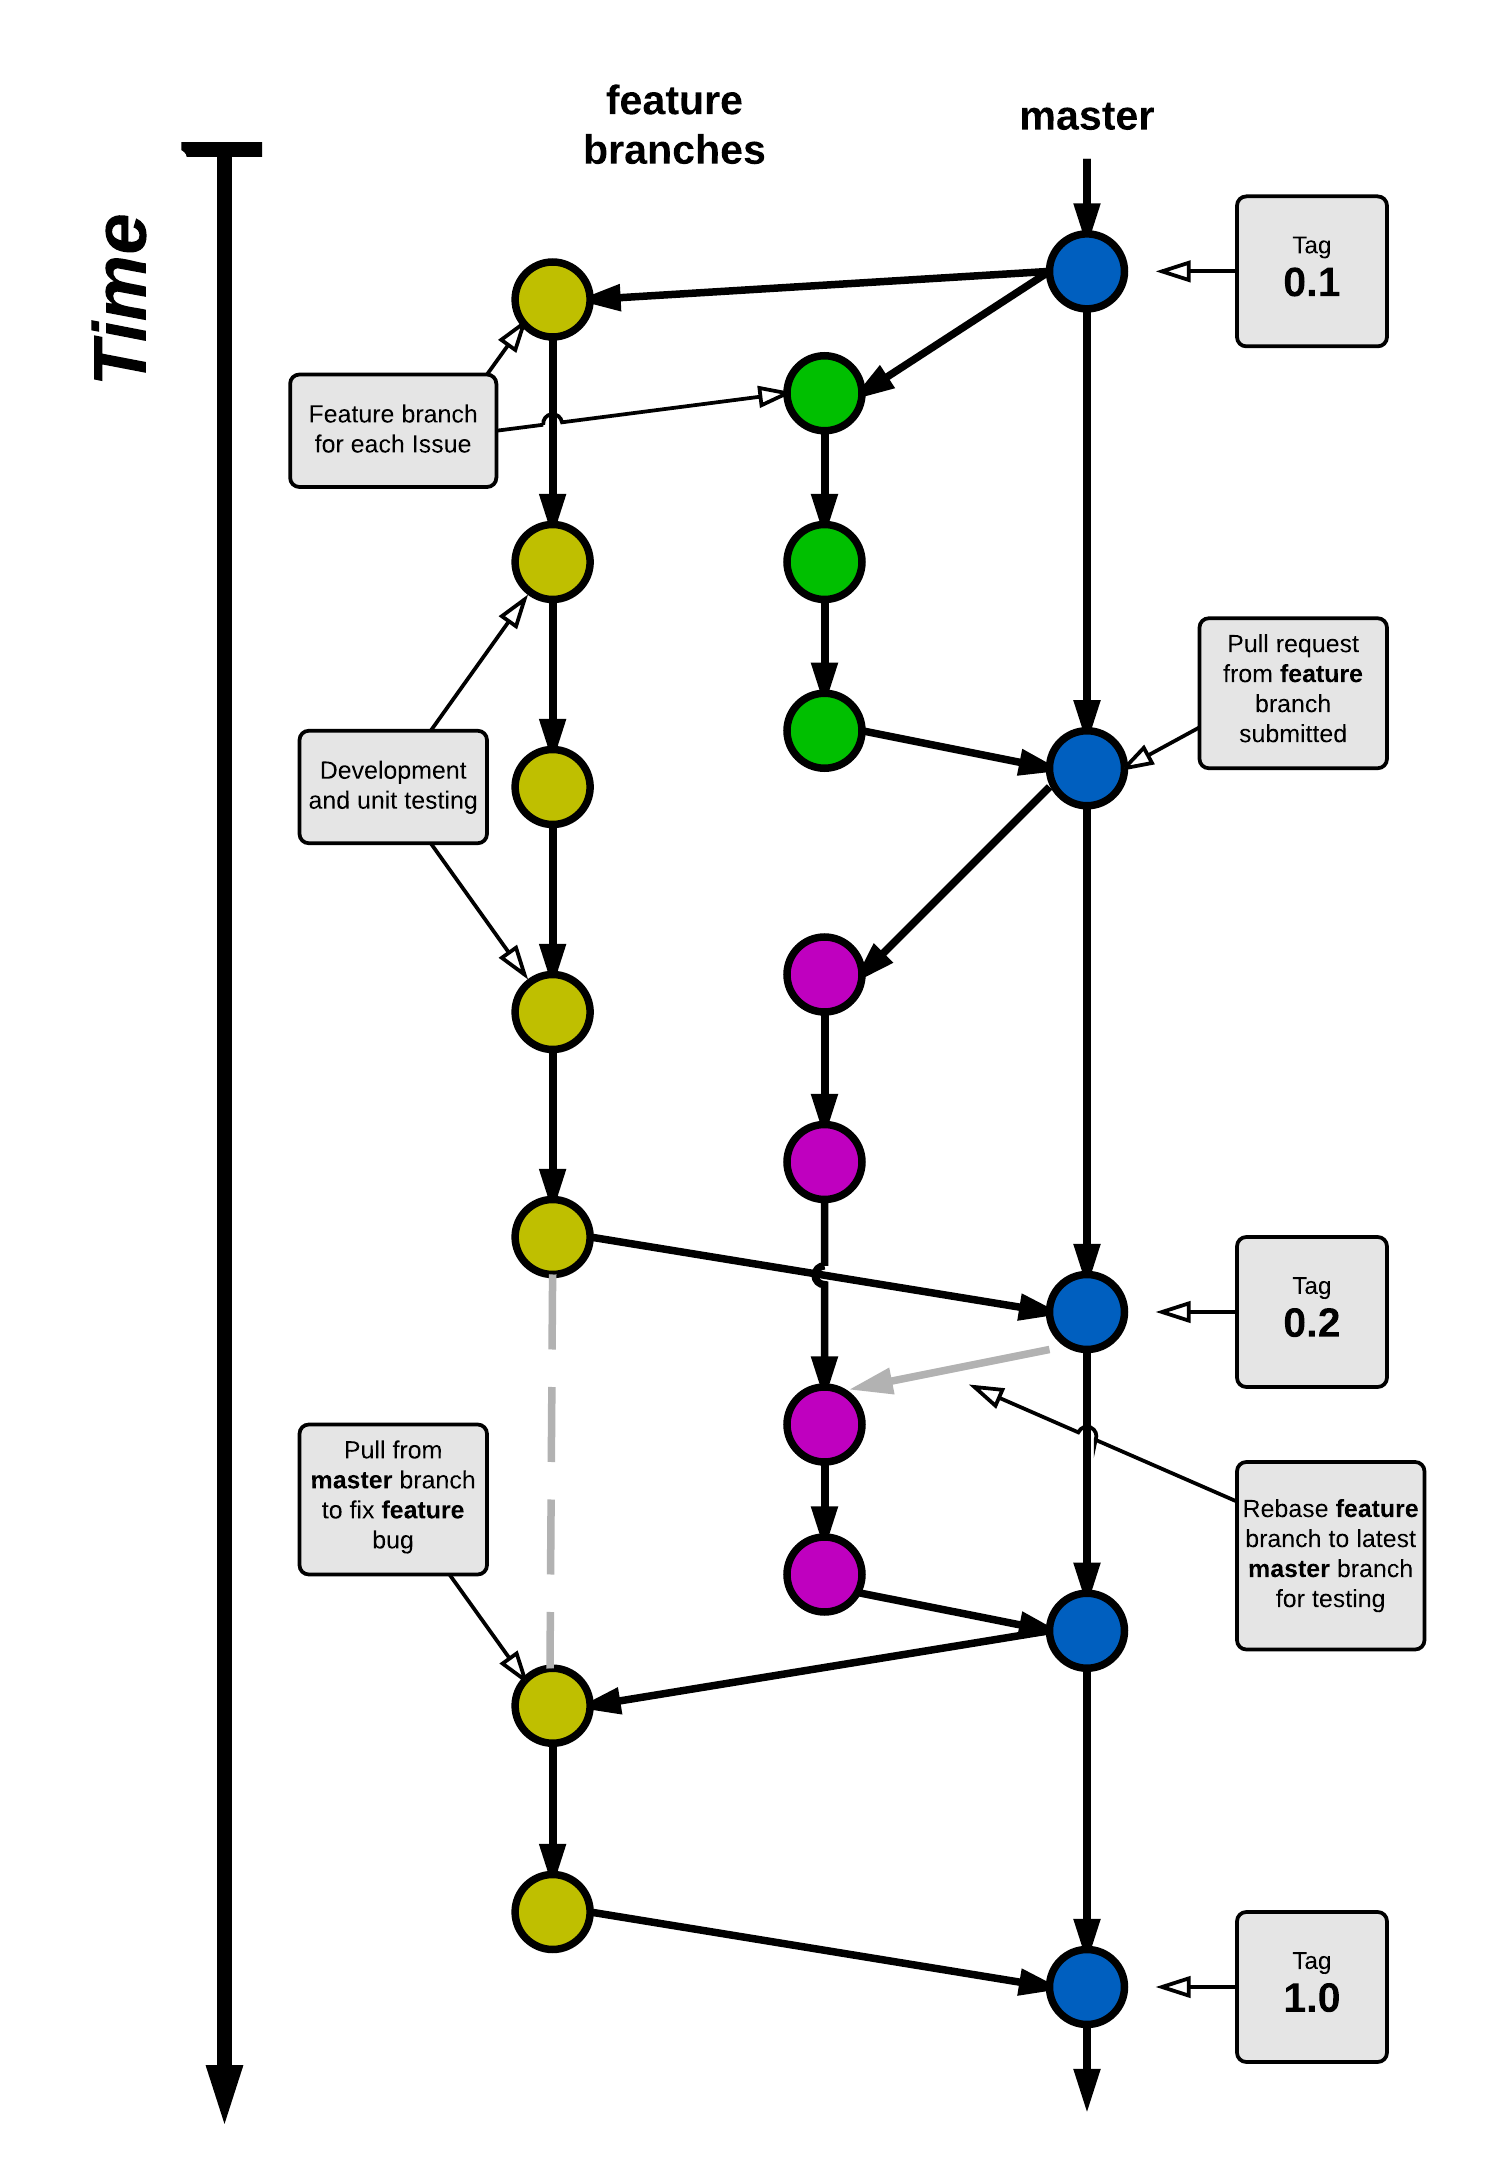
\includegraphics[width=1.0\textwidth]{version_control_model}}%
  \label{fig:versioning}
\end{figure}

\section{Design}
Fundamentally, our project and the design to complete it relies upon Abstract Syntax Tree (AST) representations of C source code and the methods in which the Clang AST parser library represents those AST trees. Therefore we have relied heavily upon documentation and research into the use of ASTs for source code evaluation and how Clang AST accomodates such use cases.

Garmin AT has previously developed infrastructure code, including a few example solutions to issues, based upon regular expression-based analysis techniques. In the process of developing additional solutions to issues, they realized that some issues cannot be accomplished through the use of regular expressions. They chose AST analysis as the more desired solution, and have since sought to use our project to both refactor current issues that could benefit from AST analysis and complete unfinished issues with either AST analysis or regular expressions (based upon the best solution possible).

Using the infrastructre developed by Garmin AT, our system will consist of the cFixer library of analysis and modification to either the AST nodes, or the source code using regular expressions, in order to resolve any code that falls outside of the standards requirements set forth within each issue (mirroring the requirements made by FAA and Garmin AT). The AST will be generated using the Clang AST parser, and accompanying library of utility code, and return all necessary results to cFixer.

With the varying nature of requirements and analysis needed at any given time, the cFixer and all input components of the system must be modular and configurable in nature. Garmin AT has already developed a set of execution-time parameters and config file structure that allows specific portions of the rulesets to be run against the provided source file, as well as passing different options and values to those rules for matching specific value requirements of the FAA and other internal code standards. We will be extending those parameters and config options as we develop additional rules for the outstanding issues.

Depending upon the desired output, either to-file or to-screen, the cFixer will log metadata regarding the status of each issue/rule function and any accompanying information necessary to convey the state of the source code before and after completion of the analysis. Writing out to file will occur in a human-readable data-interchange file format (i.e. XML, JSON, or YAML). This could potentially be updated to include a format that is suited for parsing into SQL-based databases as well, but this would be an additional requirement provided by the client and requiring additional design to complete.

\section{Tasks}
All of the primary tasks in this project revolve around implementing issues which have already been defined. Many issues have a description and number, some do not. Both sets of issues are listed in the Issues section. In addition to work on individual issues, we will need to create integration tests to ensure the functionality of checking against multiple issues at once and system tests for the functionality invoking the issue checking.

For each issue task, we will complete the following subtasks:
\begin{itemize}
	\item Team review of issue definition and requirements
	\item Individual development of issue solution
	\item Individual development of solution tests
	\item Team review of solution correctness
\end{itemize}

The team review of subtasks not only allows the team time to agree on what exactly the problem is and what the best solution for it would be, but also gives each team member the opportunity to get familiar with each issue.

\section{Risk Assessment}
One major risk that has already been identified is that our mentor and client may without much warning have to attend to personal business outside of the country and would be out of contact for questions and guidance. Right now, the contingency plan to maintain direction from Garmin AT is to have another software engineer step in as mentor.

Outside of project-shattering risks, one major functional problem that may arise is that when issues are run against a source file, they are set to either flag-and-fix or just flag problems as defined by that issue. The functional problem that arises is if two issues attempt to fix the same code, or one issue's fix creates a problem which is flagged by another issue. These sorts of conflicts are best mitigated by thorough testing and the implementation of some sort of issue priority or ordering.

Another risk that may come up is conflicts in changes to the code base. With four people potentially modifying the same code at once, merge conflicts are more than likely. To avoid this, we will implement the standard Git versioning practice of creating branches for the master version, a quality assurance version for Garmin to check off on, development, and then individual task development versions for us to modify. Issue branches will be merged back into development as work is completed and the other three branches will merged back ``up'' a level periodically. The details of this implementation are covered in the integration plan section. The general idea is that by carefully controlling what code is in which version, we not only avoid merge conflicts, but also ensure that the master version is always stable and that the QA version is a presentable version for Garmin to check.

\section{Testing}
Tests will be created for each issue to ensure that problems are correctly flagged and code corrections made (if the toolset is capable of making such corrections; if not, flagging only). Tests will accomodate both false-positive and false-negative situations; i.e. the rule incorrectly flags code that conforms to the rule, or the rule fails to flag code that does not conform to the rule.

In addition to individual issue tests, integration and system tests will be implemented to ensure that two rules do not result in race conditions, conflicting code states, or other unintended consequences such as code that is no longer able to compile.

We will rely heavily upon unit tests for validation of each methods functionality and compatability within the greater codebase. The overarching integration tests will be used to validate that the entire system completes without errors across the lifespan of an execution.

\section{Preliminary Timetable}
\noindent\begin{longtable}{| p{.20\textwidth} | p{.70\textwidth} |}
\hline
\textbf{October} & Inital meeting with client, introduction to project, development of problem statement and technology review\\
\hline
October 17 & Biweekly phone meeting with client\\
\hline
October 27 & Garmin AT On-site Meeting with mentor\\ 
\hline
\textbf{November} & Requirements gathering and initial code review\\
\hline
November 7 & Biweekly phone meeting with mentor\\
\hline
November 21 & Biweekly phone meeting with mentor\\
\hline
\textbf{December} & Individual development of solutions to three issues (9 total)\\
\hline
December 5 & Biweekly phone meeting with mentor\\
\hline
December 8 & Version 1.0 released\\
\hline
December 19 & Biweekly phone meeting with mentor\\
\hline
\textbf{January} & Individual development of solutions to two issues (6 total), reviewed and released\\
\hline
January 9 & Biweekly phone meeting with mentor\\
\hline
January 23 & Biweekly phone meeting with mentor\\
\hline
\textbf{February} & Individual development of solutions to two issues (6 total), reviewed and released\\
\hline
February 6 & Biweekly phone meeting with mentor\\
\hline
February 20 & Biweekly phone meeting with mentor\\
\hline
\textbf{March} & Individual development of solution to one issue (3 total), reviewed and released\\
\hline
March 6 & Biweekly phone meeting with mentor\\
\hline
March 13 & Version 2.0 released\\
\hline
March 20 & Biweekly phone meeting with mentor\\
\hline
\textbf{April} & Individual development of solution to two issues (6 total), reviewed and released\\
\hline
April 3 & Biweekly phone meeting with mentor\\
\hline
April 17 & Biweekly phone meeting with mentor\\
\hline
\textbf{May} & Additional development of solution to one issue (3 total) as needed and capable, quality assurance and testing given priority, presentation and documentation emphasized\\
\hline
May 1 & Biweekly phone meeting with mentor\\
\hline
May 8 & Version 3.0 released\\
\hline
May 15 & EXPO Event\\
\hline
\end{longtable}

\section{Team Roles}

Because most of the work for this project is in the issues, each member on the team will have the same role working on implementing issues, tests, and reviewing each others' issues. This means that rather than one team member owning a specific aspect of the project, each team member owns individual issues and work related to them. In the case of the non-issue based work, team members will participate in joint development and decide who performs what tasks.

\section{Integration Plan}

Although most of the infrastructure code is already in-place (developed by Garmin AT prior to the start of this project), we will be making extensive additions and extensions to that codebase. We intend to provide unit tests for all new code added to the project. Therefore once we have added, tested, and validated that the infrastructure code works as intended, our integration plan consists of adding new rules that resolve issues and validating them through the addition of unit tests. These unit tests will validate that the new functionality meets the feature requirements of the issue. These tests will utilize a mock source code file as input in order to simulate the entire lifecycle of the system.

Each issue/rule will be developed in a separate git branch that will be used for feature development, unit test development, integration testing, and validation. Once a issue/rule has been shown to conform to the requirements of the issue, we will submit a pull request from the \textit{feature} branch to the \textit{master} branch. The Garmin AT client/mentor will review each pull request and approve or reject based upon their experience and understanding of the business requirements associated with the issue/rule. After at least one issue has been merged into the \textit{master} branch, we will create minor version tags in order to manage baseline code versions from the \textit{master} branch to the in-progress \textit{feature} branches.

Testing, verification, and validation are all required during the development of a \textit{feature} branch. A \textit{feature} branch will not be considered test complete and ready for submission in a pull request to the \textit{master} branch, until it has been tested against the current \textit{master} branch codebase. Therefore we will be conducting rebasing of the \textit{feature} branches prior to testing.

This process will repeat for each subsequently scheduled major version. This process will allow us to safely and efficiently integrate each functional block of changes into the codebase without halting parallel efforts within the codebase.

\section{Dataflow Sequence Diagram}
See Figure~\ref{fig:dataflow} for the dataflow sequence diagram representing our proposed system.

\begin{figure}[hp]
  \caption{Dataflow Sequence}
	\makebox[\textwidth][c]{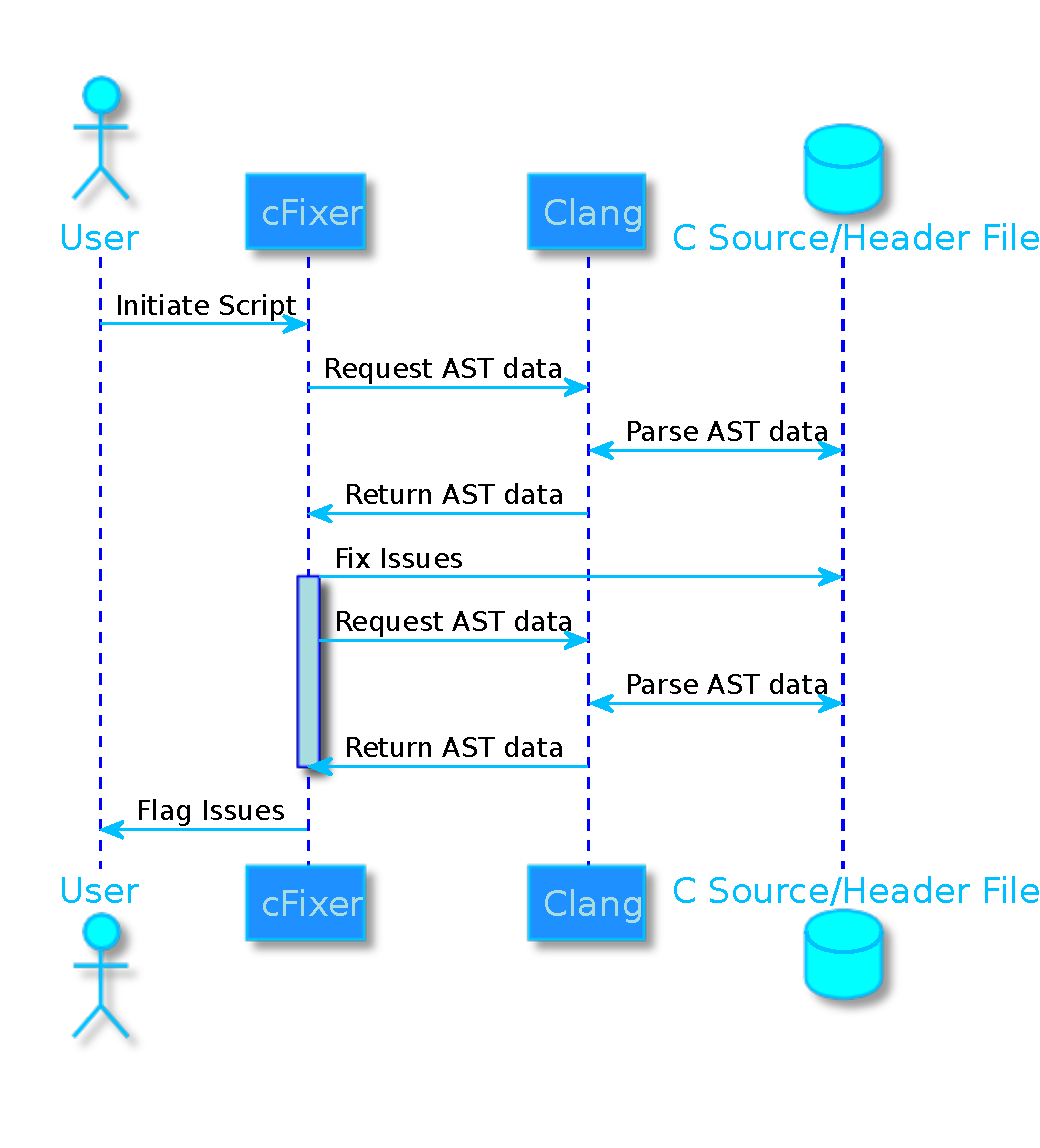
\includegraphics[width=1.2\textwidth]{dataflow}}%
  \label{fig:dataflow}
\end{figure}

\section{User Interface Requirements}

For this product, the user interface will work entirely through the command line, as this is a tool which will be integrated into the compilation and code check-in processes. The tool will take source and configuration files as input and output to either another file or the standard output. Text output should be formatted in a way that is human-readable and relatively easy to parse.


\end{document}
